\documentclass[a4paper,11pt]{article}
\usepackage[margin=2cm]{geometry}

\usepackage[titletoc,toc,title,page]{appendix}
\usepackage[nodayofweek]{datetime}
\usepackage{cite}
\usepackage{graphicx}
\longdate

\usepackage{minted}
\usepackage{titlesec}
\usepackage{hyperref}
\usepackage{fancyhdr}
\pagestyle{fancyplain}
\fancyhf{}
\lhead{\fancyplain{}{M.Sc.\ Group Project Report}}
\rhead{\fancyplain{}{\today}}
\cfoot{\fancyplain{}{\thepage}}


\title{Implementation of attentional bistability of the dragonfly visual neurons in an intelligent biomimetic agent\\\Large{--- Final Report ---}}
\author{Juan Carlos Farah, Panagiotis Almpouras, Ioannis Kasidakis, Erik Grabljevec, Christos Kaplanis\\
       \{jcf214, pa512, ik311, eg1114, ck2714\}@doc.ic.ac.uk\\ \\
       \small{Supervisors: Professor Murray Shanahan, Zafeirios Fountas, Pedro Mediano}\\
       \small{Course: CO530/533, Imperial College London}
}

\begin{document}
\section{Centrifugal Small Target
Motion Detector Neuron 1 (CSTMD1)}
\subsection{Methodology}
The function of this module is to create inhibitory effects to the output received from the point neurons of the ESTMD module  with the aim to create a meaningful output for the pattern recognition module which is then identifying spiking patterns. The main aspects we needed to consider were:
\begin{enumerate}
	\item The complicated nature of the morphologically-modelled CSTMD1
	\item The simulation environment of the CSTMD1 neurons (NEURON simulation environment)
	\item How to efficiently connect this module with both the ESTMD and the pattern recognition module
	\item Key Performance Indicators to measure the performance and the plausibility of the module
 
\end{enumerate}

Given that the CSTMD1 is multi-compartmental model with several parameters that directly or indirectly affect its activity and effect to a given input, we needed to first fully understand the given model before proceeding with any further decisions. Thus, we performed several tests in order be aware of all the plausible values that should be tried for each of the parameters.

Moreover, we had to consider what would be the best way to provide stimuli to the CSTMD1 neurons as an input from the ESTMD module. The NEURON simulation environment provides many classes as a connection to a model from an external input. After examining all the different possibilities we decided to use a leaky integrator (IntFire2() point process) 
\emph{\color{red}EXPLAIN MORE ABOUT INTFIRE2???}. More specifically, the ESTMD module provides a time series of neuron spikes which is essentially an array of values each of which corresponds to a spiking rate per retina pixel. Thus, we initiated one leaky integrator for each pixel and provided the spiking rate as its total current. We then connected these point processes to each of the CSTMD neurons used for the simulation. In order to make our model as much biologically plausible as possible, we added some randomized delays to the connections of the leaky integrators with the neurons with the aim to ensure that the desired inhibitory effect will be achieved while neurons are provided with some stimuli. We also applied a Gaussian bell to the weights of these connections, with which we achieved to have more weight to the connections corresponding to pixels of the central retinal field while these weights fade out as we move along to the peripheral area of the visual field.

With regards to the output, since the pattern recognition module requires a considerable amount of spike trains as an input, we had to find a way to connect the 2 modules without severely affecting the speed and performance of the CSTMD1 module. Hence, given the morphologically large axon of the CSTMD1 neuron (GEURTEN 2007) we decided instead of using as many neurons as the inputs required by the pattern recognition module, to apply a large number of electrodes to different compartments of the neurons and thus provide the adequate amount of spike trains without limiting the biological plausibility of our model.

After successfully connecting the different modules, our next goal was to define key performance indicators for the CSTMD1 module in order to measure as accurately as possible its performance and also be able to modify the several parameters of the given model and observe their effect to the simulation. For this purpose, we created several plots which recorded the activity of different compartments of the neurons as well as their spiking rates. 
\newpage
\begin{figure}
\centering
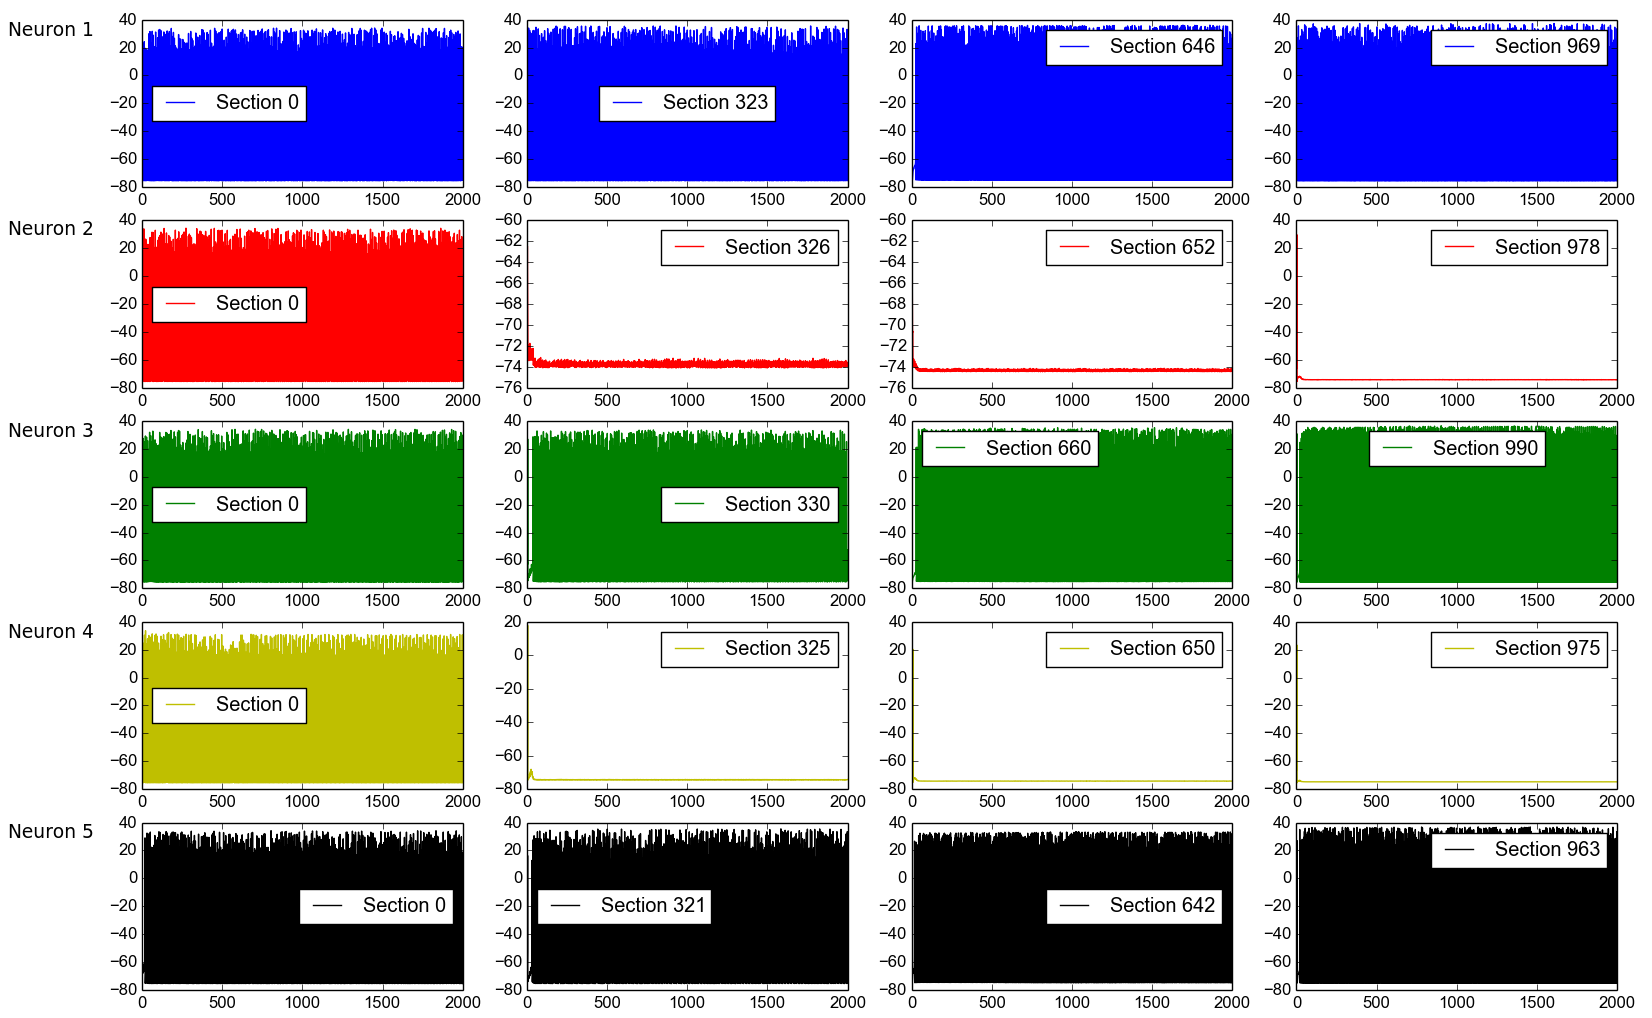
\includegraphics[scale = 0.3]{compartments}
\caption{Compartmental activity in a CSTMD1 neuron simulation showing inhibitory effects}
\end{figure}



We also extended the module to be able to run several simulations while given different inputs from the ESTMD module so as to observe if there is any evidence that our CSTMD1 module, when presented with two targets in the visual receptive field, would select one of them as we expected. However, after modifying all the possible parameters and trying different inputs, we observed that the CSTMD1 model is not
displaying this selectivity.

The web client \emph{\color{red}(MULTI SIMULATIONS????????????)} that we introduced supports running simulations of the CSTMD1 module. We transferred all the functionality as described above and thus the user is able to change all the significant parameters of the model and observe the resulting CSTMD1 neurons' behaviour as well as the behaviour of KPIs in the model.

\end{document}